
\label{cap:desen}
O principal objetivo deste trabalho é estudar e comparar os algoritmos de boosting em 4 datasets diferentes e analisar a influência dos hiperparâmetros no modelo. O estudo será feito com os parâmetros \textit{Default} de cada algoritmo, depois alguns deles serão alterados e, por final, utilizaremos o Optuna para otimizá-los.

O objetivo da escolha dos conjuntos de dados se baseou em analisar o comportamento dos modelos construídos e dos hiperparâmetros em conjuntos de dados com propriedades distintas, como por exemplo maior presença de variáveis categóricas ou apenas variáveis numéricas.

Nas próprias seções, será abordada uma visão geral da metodologia, uma análise dos conjuntos de dados e as implementações no \textit{jupyter-notebook}.

\section{Bibliotecas e Ferramentas}
Todo o pipeline de estudo e análise é feito usando Python 3.8.8. No código final no GitHub será detalhado todas as versões em um arquivo \textit{requeriments.txt}, mas de modo geral as principais bibliotecas utilizadas nesse estudo são:
\begin{itemize}
    \item \textbf{numpy:} biblioteca em python para trabalhar com arrays n-dimensional e algumas funções matemáticas de álgebra linear.
    \item \textbf{pandas:} biblioteca em python utilizada para manipulação e análise de conjunto de dados e séries temporais.
    \item \textbf{matplotlib:} biblioteca em python para visualização de dados.
    \item \textbf{seaborn:} biblioteca em python para visualização de dados baseada no \textbf{matplotlib:}.
    \item \textbf{scipy:} biblioteca em python de pacote científico computacional
    \item \textbf{sys:} biblioteca que oferece funções e variáveis usadas para manipular diferentes partes do ambiente e do tempo de execução do python.
    \item \textbf{timeit:} biblioteca para medir o tempo de execução de programas python.
    \item \textbf{gc:} é o garbage collector utilizado nas linguagens de programação para rastrear os objetos na memória.
    \item \textbf{sklearn:} biblioteca de aprendizado de máquina em python.
    \item \textbf{xgboost:} biblioteca do XGBoost.
    \item \textbf{catboost:} biblioteca do CatBoost.
    \item \textbf{lightbm:} biblioteca do LightGBM.
    \item \textbf{optuna:} biblioteca do Optuna.
    \item \textbf{shap:} biblioteca do SHAP.
\end{itemize}

\section{Data Cleaning, Data Preparation e Análise Descritiva}
Nesta seção iremos fazer uma breve descrição dos conjuntos de dados, análise descritivas das variáveis e a distribuição nos conjuntos de dados. Primeiramente, precisamos ajustar dados que foram inseridos incorretamente, lidar com os valores \textit{missing} e realizar as transformações, ou conversões, das variáveis para cada modelo, por exemplo variáveis categóricas para numéricas no caso do LightGBM e XGBoost. 
Todas as análises nos conjunto de dados seguem a mesma metodologia: identificar o tipo de cada coluna (int, float, str) verificar se existem valores \textit{missing} e realizar as transformações ou criações de variáveis para cada modelo.

Serão utilizados 4 conjunto de dados diferentes para este estudo, todos eles podem ser encontrados no \href{https://www.openml.org/}{OpenML}, \href{https://www.kaggle.com/}{Kaggle} ou \href{https://archive.ics.uci.edu/ml/index.php}{UCI Machine Learning Repository}. 
\subsection{Diabetes}
O primeiro conjunto de dados é o \href{https://www.kaggle.com/datasets/tigganeha4/diabetes-dataset-2019}{Diabetes Dataset 2019}
Este conjunto de dados é originalmente do \textit{Prediction of Type 2 Diabetes using Machine Learning Classification Methods}. O objetivo é prever, com base em medidas de diagnóstico, se um paciente tem diabetes. As variáveis são:
\begin{itemize}
    \item \textbf{Idade:} idade faixa de anos.
    \item \textbf{Sexo:} sexo do paciente [M: Masculino, F: Feminino].
    \item \textbf{Diabetes na Família:} se tem diabetes no histórico familiar.
    \item \textbf{Pressão Alta:} se o paciente possui pressão alta.
    \item \textbf{Atividade Física:} se pratica atividade física.
    \item \textbf{IMC:} índice de massa corporal (peso em $kg$/(altura em $m$)$^2$).
    \item \textbf{Fumante:} indica se o paciente é fumante.
    \item \textbf{Alcoólatra:} indica se o paciente é alcoólatra.
    \item \textbf{Horas de sono:} quantidade de horas de sono
    \item \textbf{Sono Profundo:} horas de sono profundo.
    \item \textbf{Medicamentos Regulares:} indica se o paciente utiliza medicamentos
    \item \textbf{JunkFood:} se o paciente consome comidas gordurosas.
    \item \textbf{Stress:} stress do paciente.
    \item \textbf{BPLevel:} nível da pressão arterial.
    \item \textbf{Gravidezes:} número de gravidezes.
    \item \textbf{Pdiabetes:} se possui pré-diabetes.
    \item \textbf{Frequência Urinaria:} frequência urinaria.
    \item \textbf{Resultado:} variável alvo (0 ou 1), se possui ou não possui diabete.
    
\end{itemize}
O primeiro passo é identificar o nome de cada coluna, seus atributos e os valores \textit{NaN} em cada linha de cada coluna. E para as variáveis numéricas uma análise descritiva, média, desvio padrão, contagem, mínimo e máximo e os quantis (25,50,75).
 
\begin{table}[H]
\begin{subtable}[c]{0.5\textwidth}
\label{descritivo:diabete}
\centering
\begin{tabular}{|c|c|c|}
 \hline
\textbf{Coluna} & \textbf{dtypes} & \textbf{\textit{NaN}}\\
  \hline
Age                &  object & 0\\
\hline
Gender             &  object & 0\\
\hline
Family\_Diabetes   &   object & 0 \\
\hline
highBP             &  object & 0 \\
\hline
PhysicallyActive   &  object & 0 \\
\hline
BMI                & float64 & 4 \\
\hline
Smoking            &  object & 0 \\
\hline
Alcohol            &  object & 0 \\
\hline
Sleep              &   int64 & 0 \\
\hline
SoundSleep         &   int64 & 0 \\
\hline
RegularMedicine    &  object & 0 \\
\hline
JunkFood           &  object & 0 \\
\hline
Stress             &  object & 0 \\
\hline
BPLevel            &  object & 0 \\
\hline
Pregancies         & float64 & 42 \\
\hline
Pdiabetes          &  object & 1 \\
\hline
UriationFreq       &  object & 0 \\
\hline
Diabetic           &  object & 1 \\
\hline
\end{tabular}
\subcaption{Tabela com o tipo de cada variável e quantidade de linhas \textit{NaN} em cada coluna.}
\end{subtable}
\begin{subtable}[c]{0.5\textwidth}
\centering
\begin{tabular}{|c|c|c|c|c|}
\hline
	& \textbf{BMI}	& \textbf{Sleep}	& \textbf{SoundSleep}	& \textbf{Pregancies}\\
\hline
\textbf{count}	& 948	& 952	& 952	& 910 \\
\hline
\textbf{mean}	& 25.7637	& 6.9495	& 5.4957	& 0.3868 \\
\hline
\textbf{std}	    & 5.4025	& 1.2731	& 1.8656	& 0.9094 \\
\hline
\textbf{min}	    & 15	& 4	& 0	& 0 \\
\hline
\textbf{25\%}	& 22	& 6	& 4	& 0 \\
\hline
\textbf{50\%}	& 25	& 7	& 6	& 0 \\
\hline
\textbf{75\%}	& 29	& 8	& 7	& 0 \\
\hline
\textbf{max}	    & 45	& 11	& 11	& 4 \\
\hline
\end{tabular}
\subcaption{Estatística descritiva das variáveis numéricas.}
\end{subtable}
\caption{Descritivo das variáveis no conjunto de dados Diabetes.}
\end{table}

Precisamos realizar um tratamento nessas linhas com \textit{NaN} e na variável resposta, Diabetic, transformando ela em 0 ou 1. Após isso devemos conferir as variáveis categorias estão escritas corretamente e podemos analisar a distribuição de algumas variáveis na população com diabete e sem diabete.


\begin{figure}[H]
 \caption{População com Diabetes e sem Diabetes.}.
 \label{fig:pop:targ:dia}
 \centering
 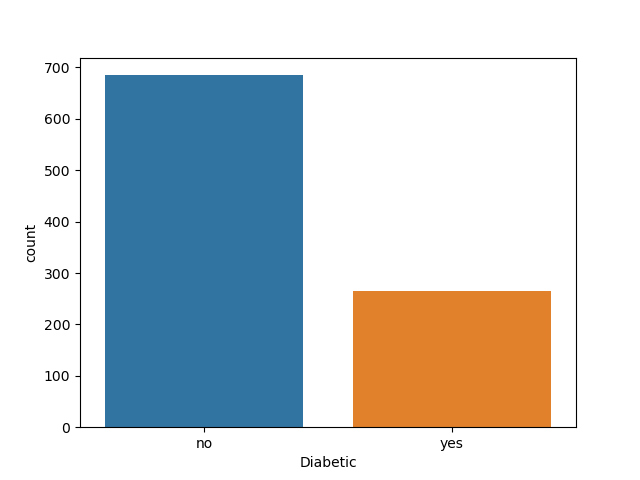
\includegraphics[scale=0.4]{images/diabete_tot.png}
\end{figure}


\begin{figure}[H]
 \caption{Distribuição das Variáveis categóricas no conjunto de dados de Diabetes.}
 \label{fig:var:cat:1:diab}
 \centering
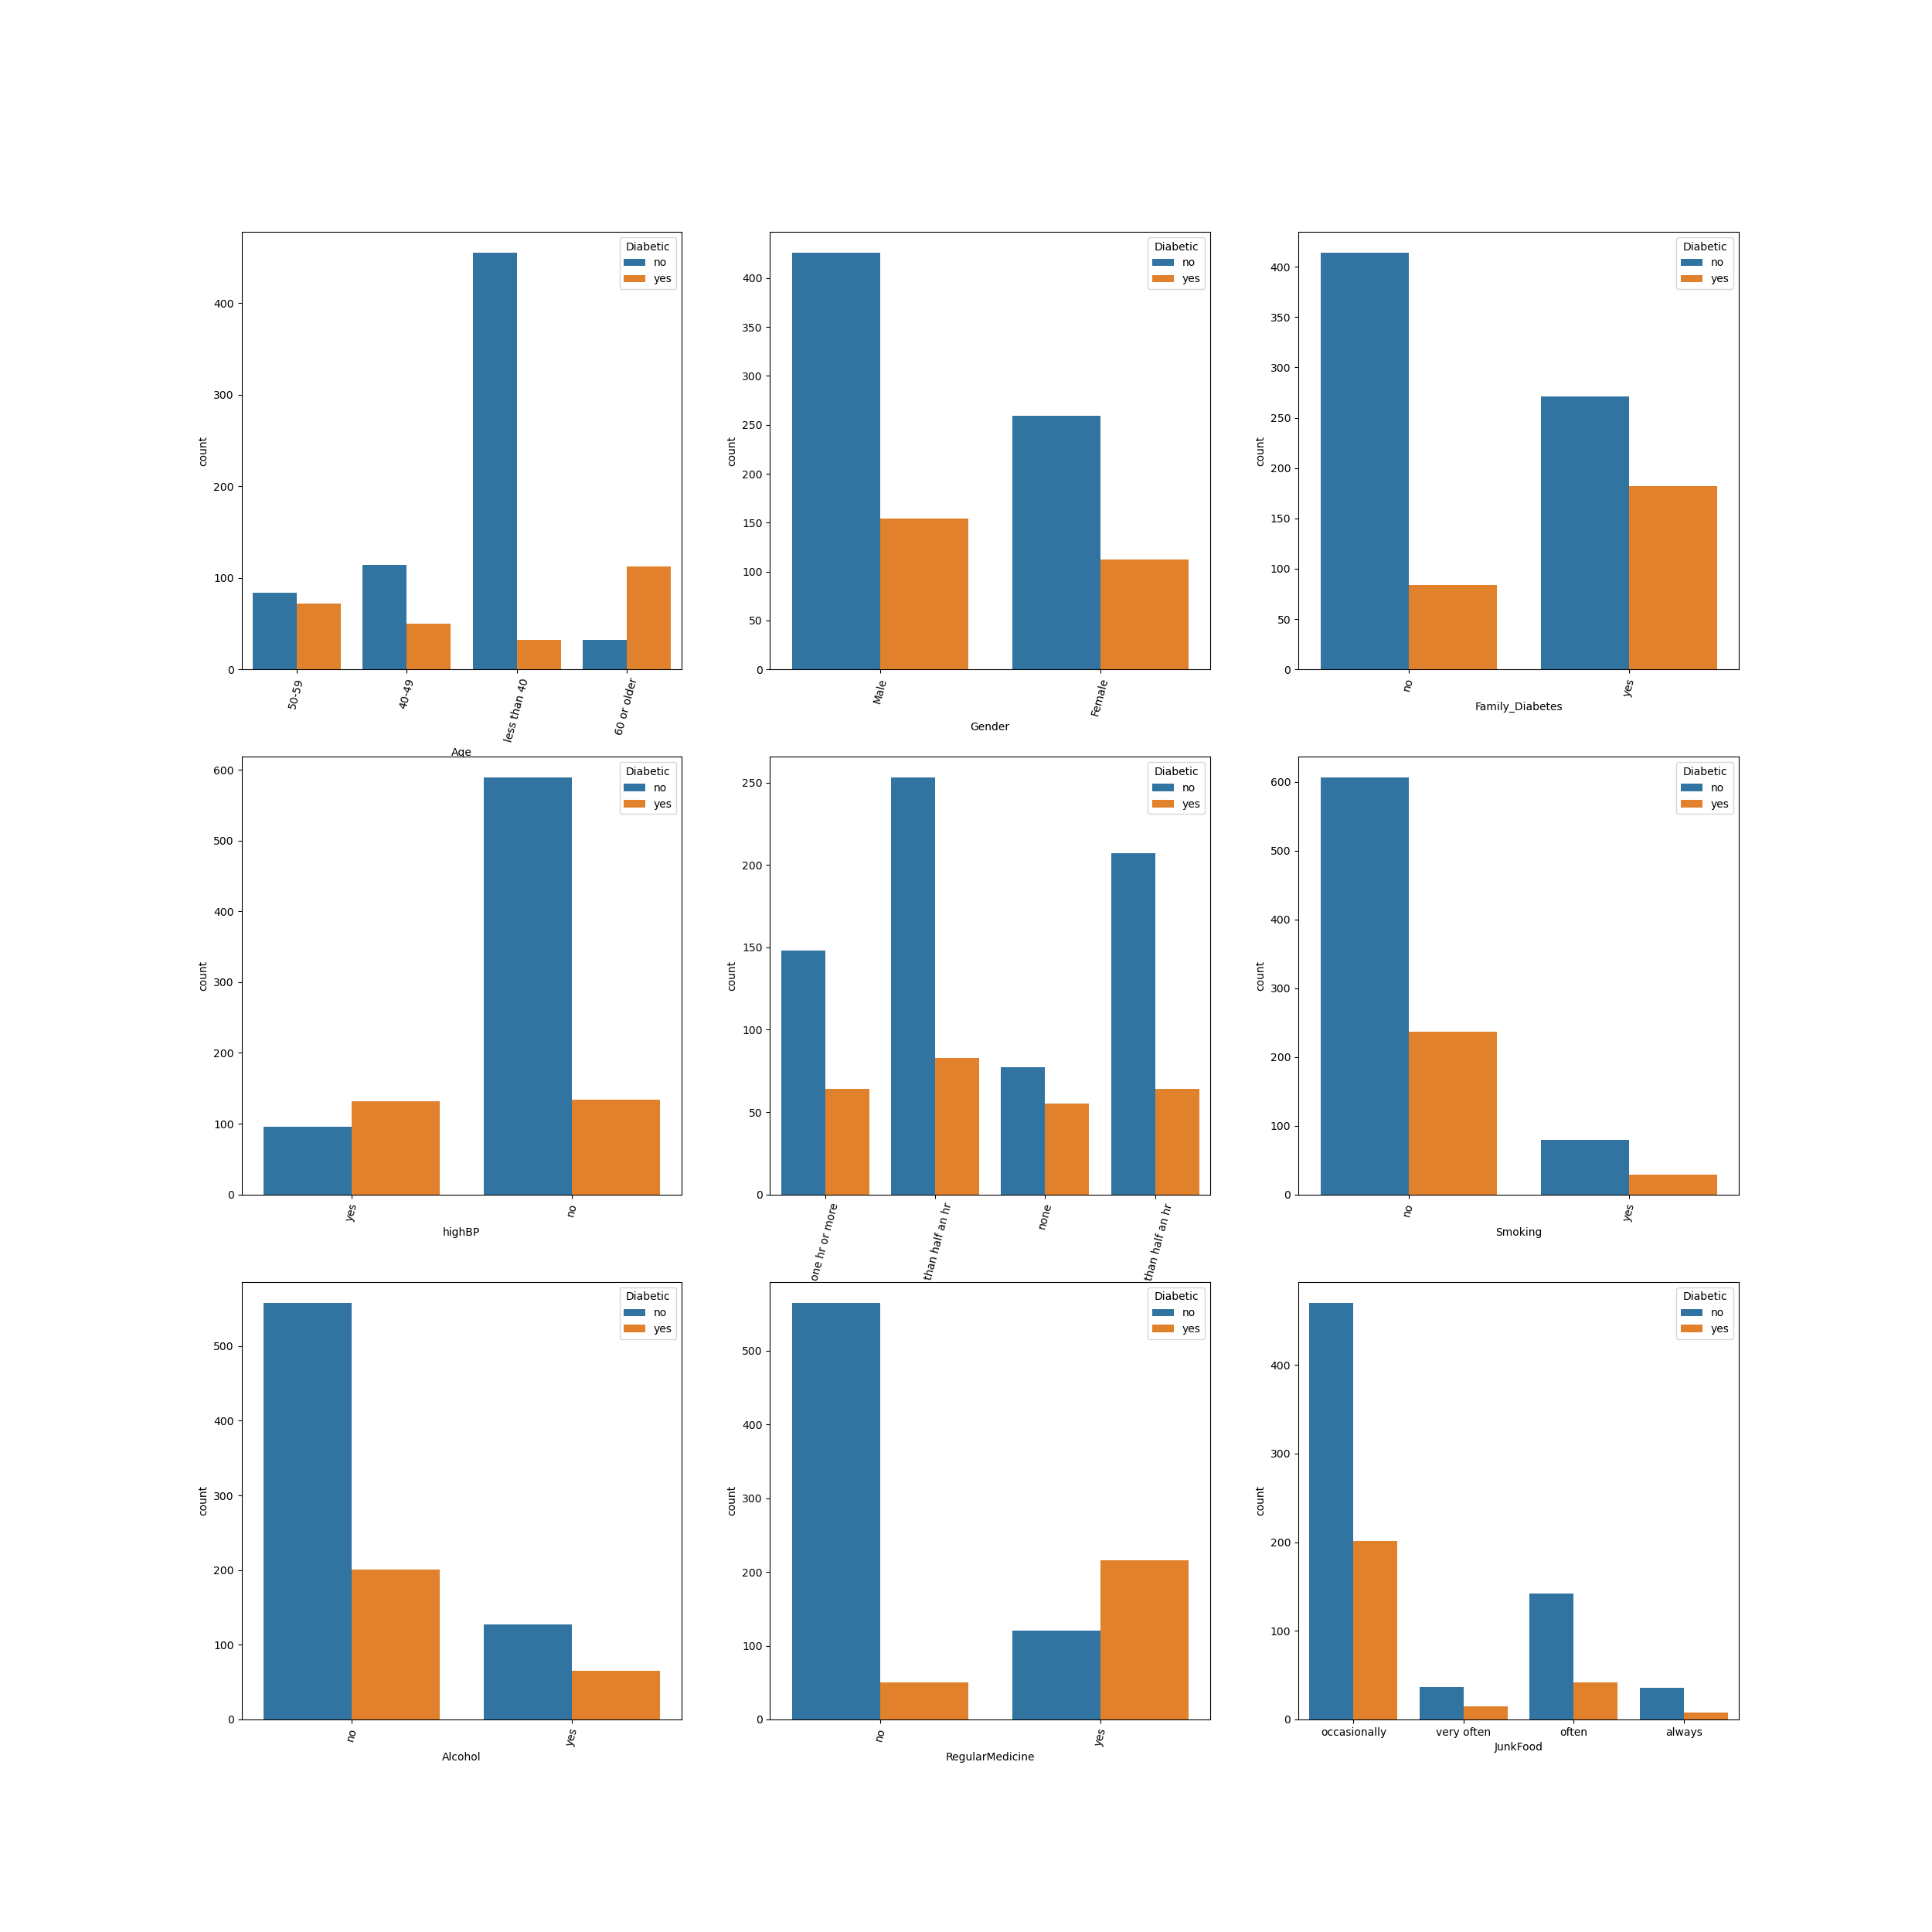
\includegraphics[scale=0.2]{images/diabete_desc.png}
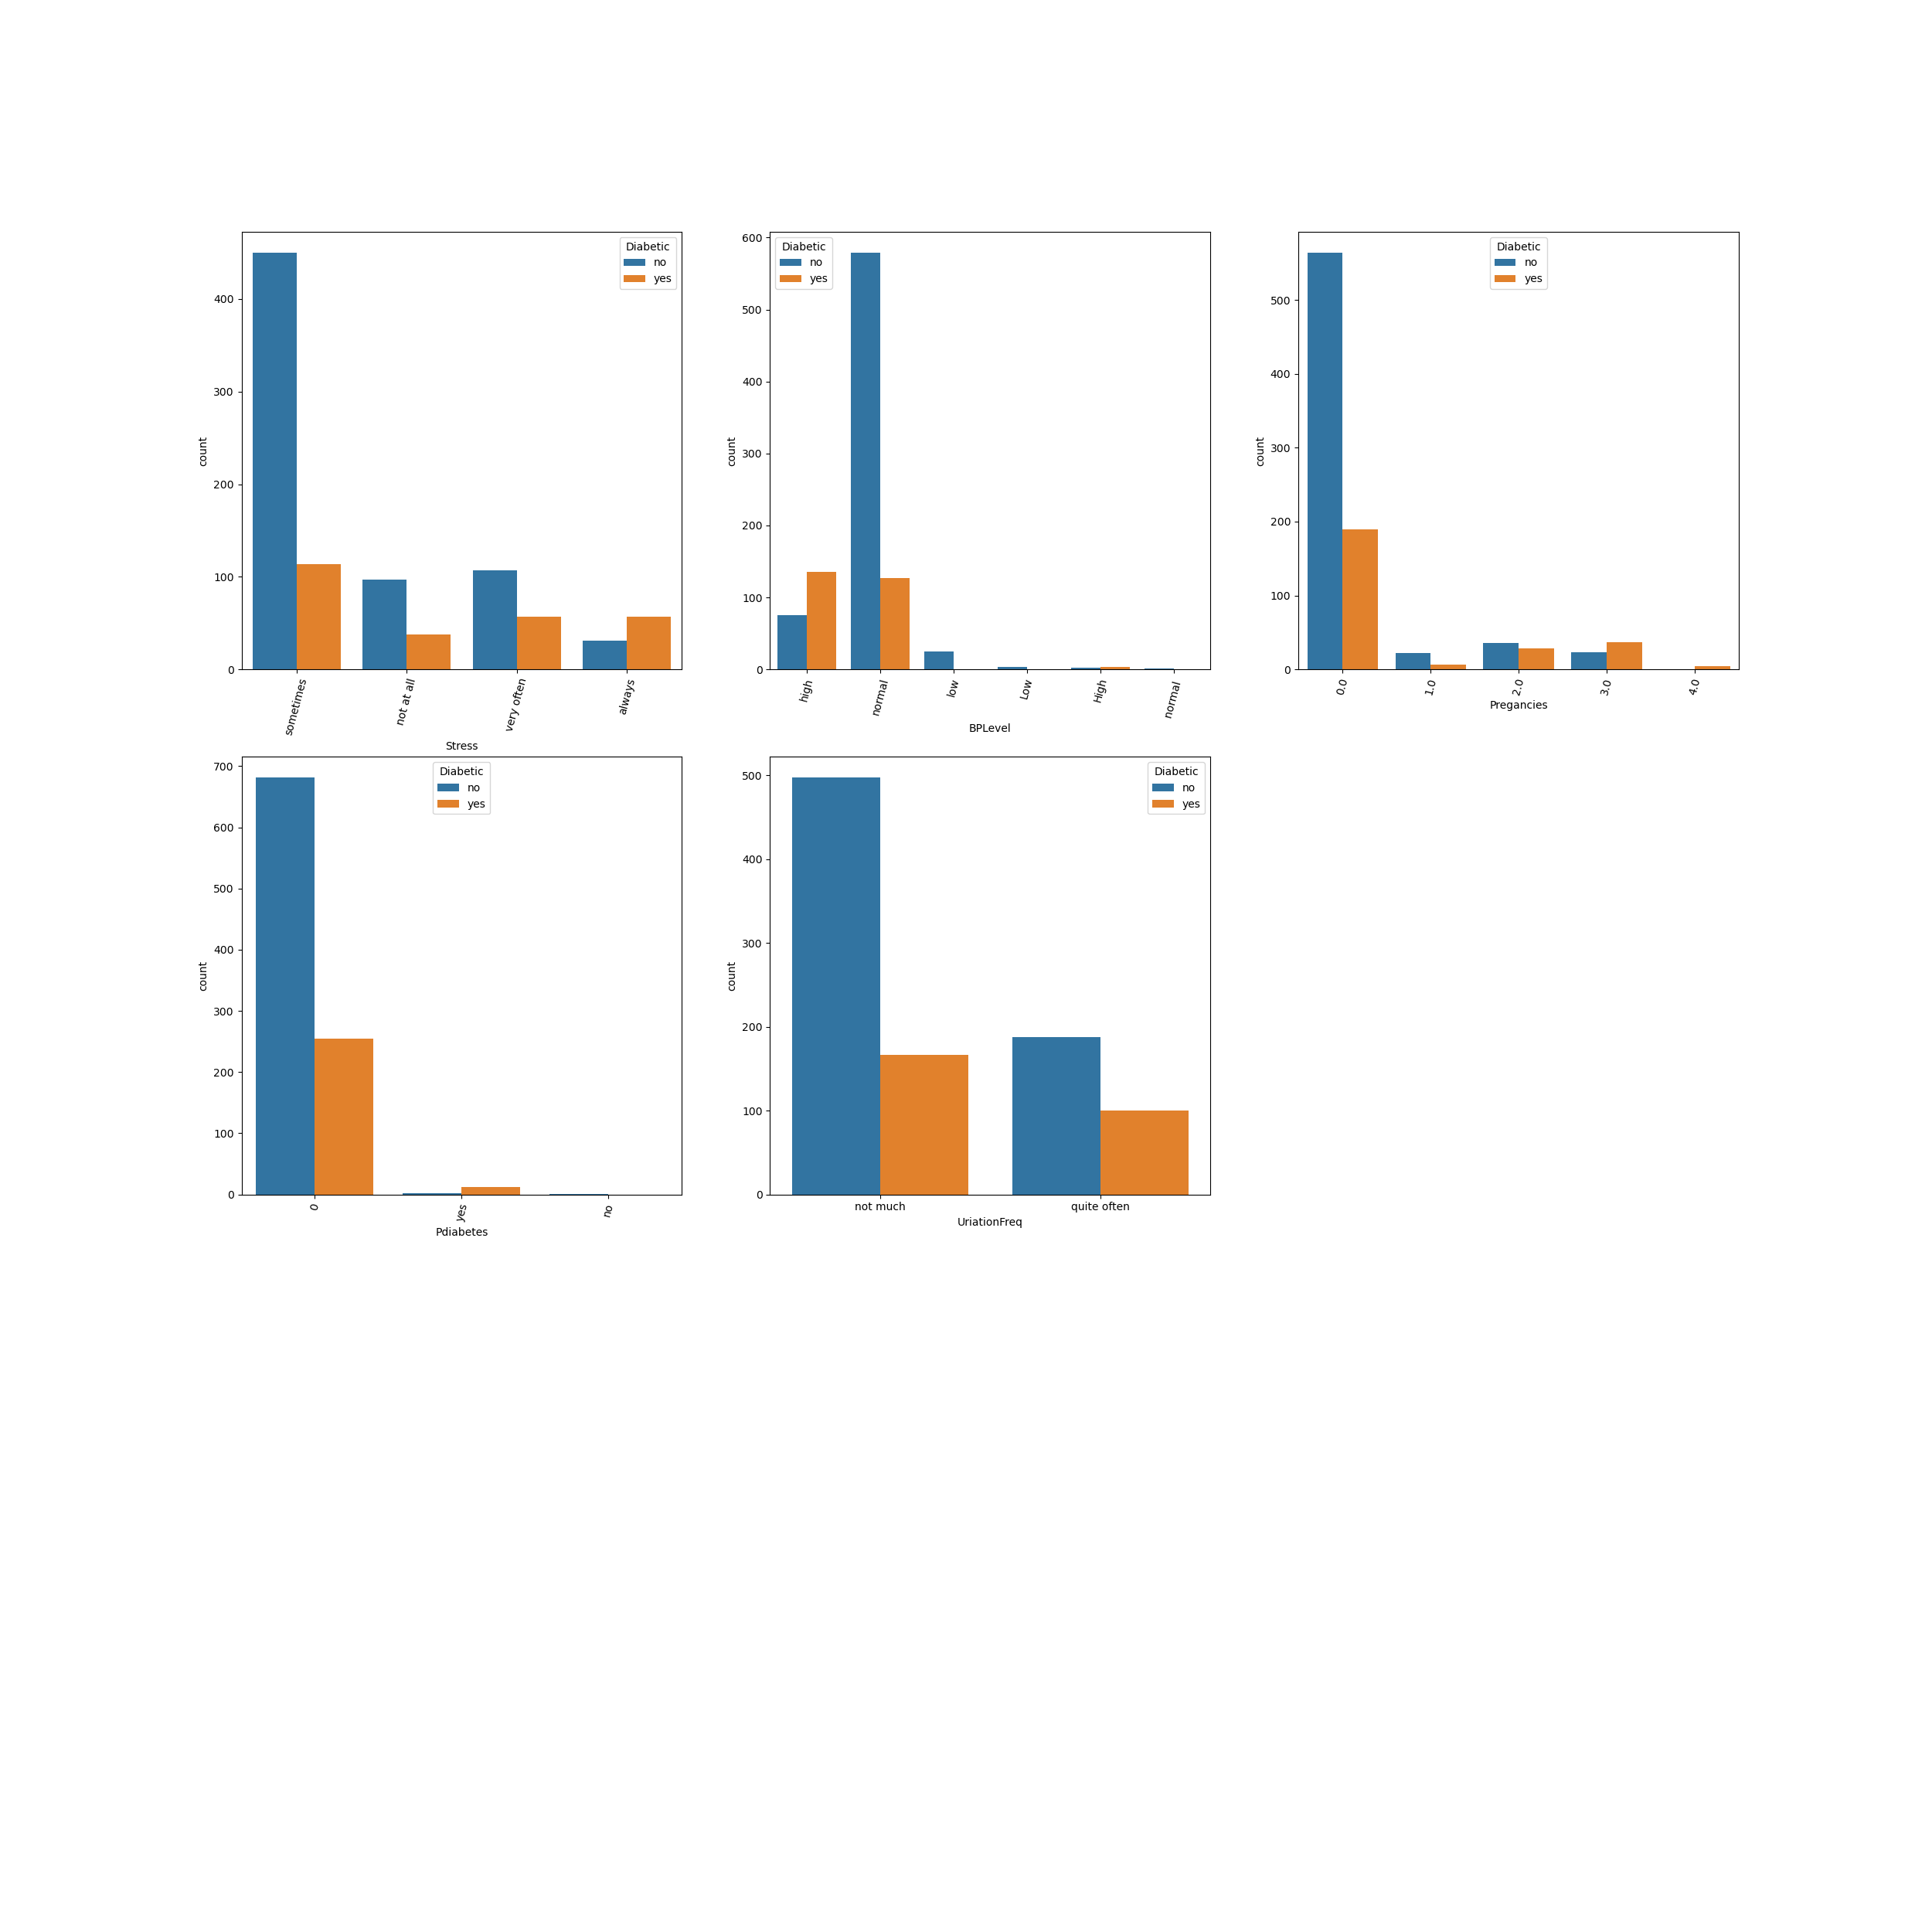
\includegraphics[scale=0.2]{images/diabete_desc_2.png}
\end{figure}


\begin{figure}[H]
     \centering
     \begin{subfigure}[b]{0.3\textwidth}
         \ \caption{Histograma das variáveis numéricas na população total.}
 \label{fig:var:1:diab}
 \centering
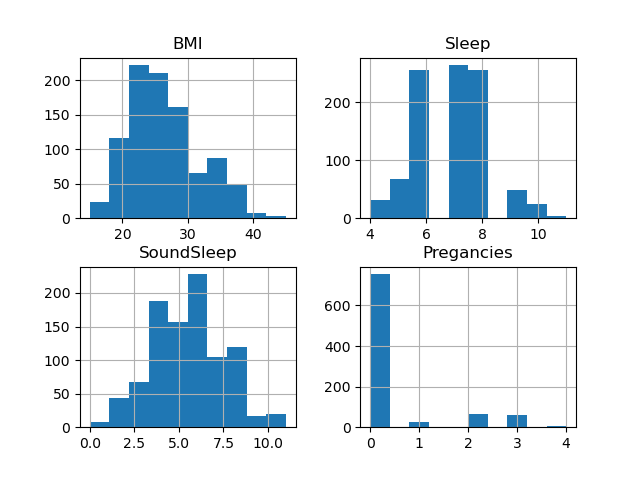
\includegraphics[scale=0.3]{images/hist_diabete.png}
     \end{subfigure}
     \hfill
     \begin{subfigure}[b]{0.3\textwidth}
         \centering
         \caption{Histograma das variáveis numéricas na população com Diabete.}
 \label{fig:var:2:diab}
 \centering
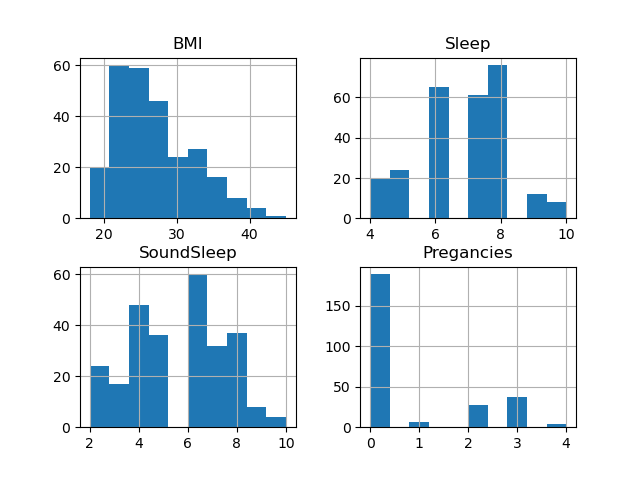
\includegraphics[scale=0.3]{images/hist_diabete_yes.png}
     \end{subfigure}
     \hfill
     \begin{subfigure}[b]{0.3\textwidth}
 \caption{Histograma das variáveis numéricas na população sem Diabete.}
 \label{fig:var:3:diab}
 \centering
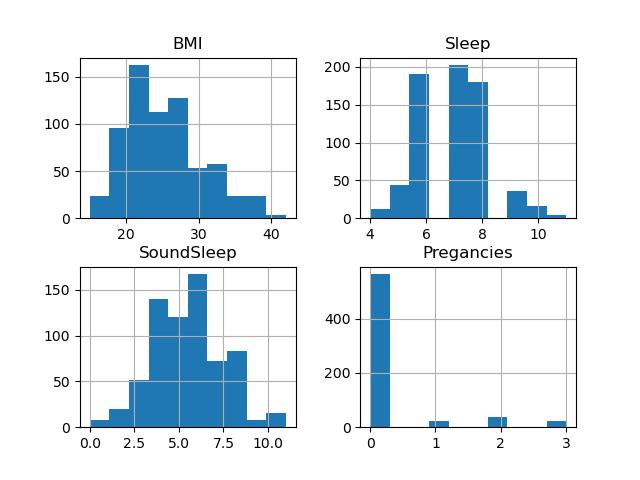
\includegraphics[scale=0.3]{images/hist_diabete_no.png}
     \end{subfigure}
        \caption{Distribuição das variáveis numéricas no conjunto de dados de Diabetes.}
         \label{fig:var:diab:t}
\end{figure}


A próxima etapa consistirá em dividir esse conjunto de dados em dois, o primeiro é com as próprias variáveis categóricas para o CatBoost enquanto que para o modelo do LightGBM e XGBoost iremos transformar as variáveis em ordinais ou utilizaremos \textit{one\_hot\_enconding}. A partir disto já teremos os nossos conjuntos de dados para o treinamento dos modelos.
\subsection{Insuficiência Cardíaca}
O segundo conjunto de dados é o \href{https://www.kaggle.com/datasets/fedesoriano/heart-failure-prediction}{Heart Failure Prediction Dataset}
Este conjunto de dados foi criado combinando diferentes conjuntos de dados já disponíveis de forma independente, mas não combinados antes. Neste conjunto de dados, 5 conjuntos de dados cardíacos são combinados em 11 características comuns. O objetivo é identificar a insuficiência cardíaca com base nas seguintes variáveis:
\begin{itemize}
    \item \textbf{Sexo:} sexo do paciente [M: Masculino, F: Feminino].
    \item \textbf{TipoDorPeito:} tipo de dor no peito.
    \item \textbf{Pressão arterial em repouso:} pressão arterial em repouso (mmHg).
    \item \textbf{Colesterol:} colesterol sérico[mm/dl]
    \item \textbf{JejumBS:} açúcar no sangue em jejum [1: se JejumBS > 120 mg/dl, 0: caso contrário].
    \item \textbf{ECG em repouso::} resultados do eletrocardiograma em repouso [Normal: Normal, ST: com anormalidade da onda ST-T (inversões da onda T e/ou elevação ou depressão do ST $>$ 0,05 mV).
    \item \textbf{HVE:} mostrando hipertrofia ventricular esquerda provável ou definitiva pelos critérios de Estes]
    \item \textbf{MaxHR:} frequência cardíaca máxima alcançada [Valor numérico entre 60 e 202].
    \item \textbf{ExerciseAngina:} angina induzida por exercício [S: Sim, N: Não].
    \item \textbf{Oldpeak:} oldpeak = ST [Valor numérico medido na depressão].
    \item \textbf{ST\_Slope:} a inclinação do segmento ST do exercício de pico [Up: ascendente, Flat: plano, Down: descendente].
    \item \textbf{Idade:} idade em anos.
    \item \textbf{Resultado:} variável alvo (0 ou 1), se possui ou não possui insuficiência cardíaca.
\end{itemize}

\begin{table}[H]
\label{descritivo:heart}
\centering
\begin{tabular}{|c|c|c|}
\hline
\textbf{Coluna} & \textbf{dtypes} & \textbf{\textit{NaN}}\\
\hline
Age              &   int64 & 0\\
\hline
Sex              &  object & 0\\
\hline
ChestPainType    &  object & 0\\
\hline
RestingBP        &   int64 & 0\\
\hline
Cholesterol      &   int64 & 0\\
\hline
FastingBS        &   int64 & 0\\
\hline
RestingECG       &  object & 0\\
\hline
MaxHR            &   int64 & 0\\
\hline
ExerciseAngina   &  object & 0\\
\hline
Oldpeak          & float64 & 0\\
\hline
ST\_Slope        &   object & 0\\
\hline
HeartDisease     &   int64 & 0\\
\hline
\end{tabular}
\caption{Tabela com o tipo de cada variável e quantidade de linhas \textit{NaN} em cada coluna no conjunto de dados de Insuficiência Cardíaca.}
\end{table}
\begin{table}[H]
\label{descritivo:heart2}
\centering
\begin{tabular}{|c|c|c|c|c|c|c|c|}
\hline
& \textbf{Age}	& \textbf{RestingBP}	& \textbf{Cholesterol}	& \textbf{FastingBS}	& \textbf{MaxHR}	& \textbf{Oldpeak}	& \textbf{HeartDisease} \\
 \hline
\textbf{count}	& 918.000	& 918.000	& 918.000	& 918.000	& 918.000	& 918.000	& 918.000 \\
 \hline
\textbf{mean}	& 53.511	& 132.397	& 198.800	& 0.233	& 136.809	& 0.887	& 0.553 \\
 \hline
\textbf{std}	    & 9.433	& 18.514	& 109.384	& 0.423	& 25.460	& 1.067	& 0.497 \\
 \hline
\textbf{min}	    & 28.000	& 0.000	& 0.000	& 0.000	& 60.000	& -2.600	& 0.000 \\
 \hline
\textbf{25\%}	& 47.000	& 120.000	& 173.250	& 0.000	& 120.000	& 0.000	& 0.000 \\
 \hline
\textbf{50\%}	& 54.000	& 130.000	& 223.000	& 0.000	& 138.000	& 0.600	& 1.000 \\
 \hline
\textbf{75\%}	& 60.000	& 140.000	& 267.000	& 0.000	& 156.000	& 1.500	& 1.000 \\
 \hline
\textbf{max}	    & 77.000	& 200.000	& 603.000	& 1.000	& 202.000	& 6.200	& 1.000 \\
\hline
\end{tabular}
\caption{Estatística descritiva das variáveis numéricas no conjunto de dados de Insuficiência Cardíaca.}
\end{table}
Neste conjunto de dados não precisamos fazer nenhum tratamento, pois os valores foram inseridos corretamente e não temos \textit{missing}.
\begin{figure}[H]
 \caption{População com Insuficiência Cardíaca e sem Insuficiência Cardíaca.}.
 \label{fig:pop:targ:card}
 \centering
 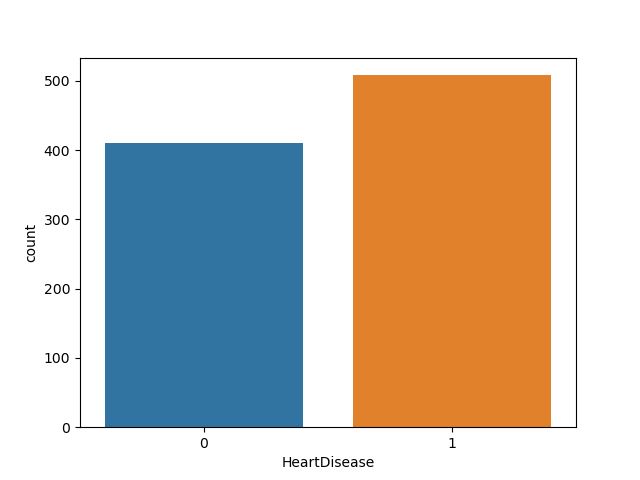
\includegraphics[scale=0.3]{images/heart_tot.png}
\end{figure}


\begin{figure}[H]
 \caption{Distribuição das variáveis categóricas no conjunto de dados de Insuficiência Cardíaca.}
 \label{fig:var:cat:1:card}
 \centering
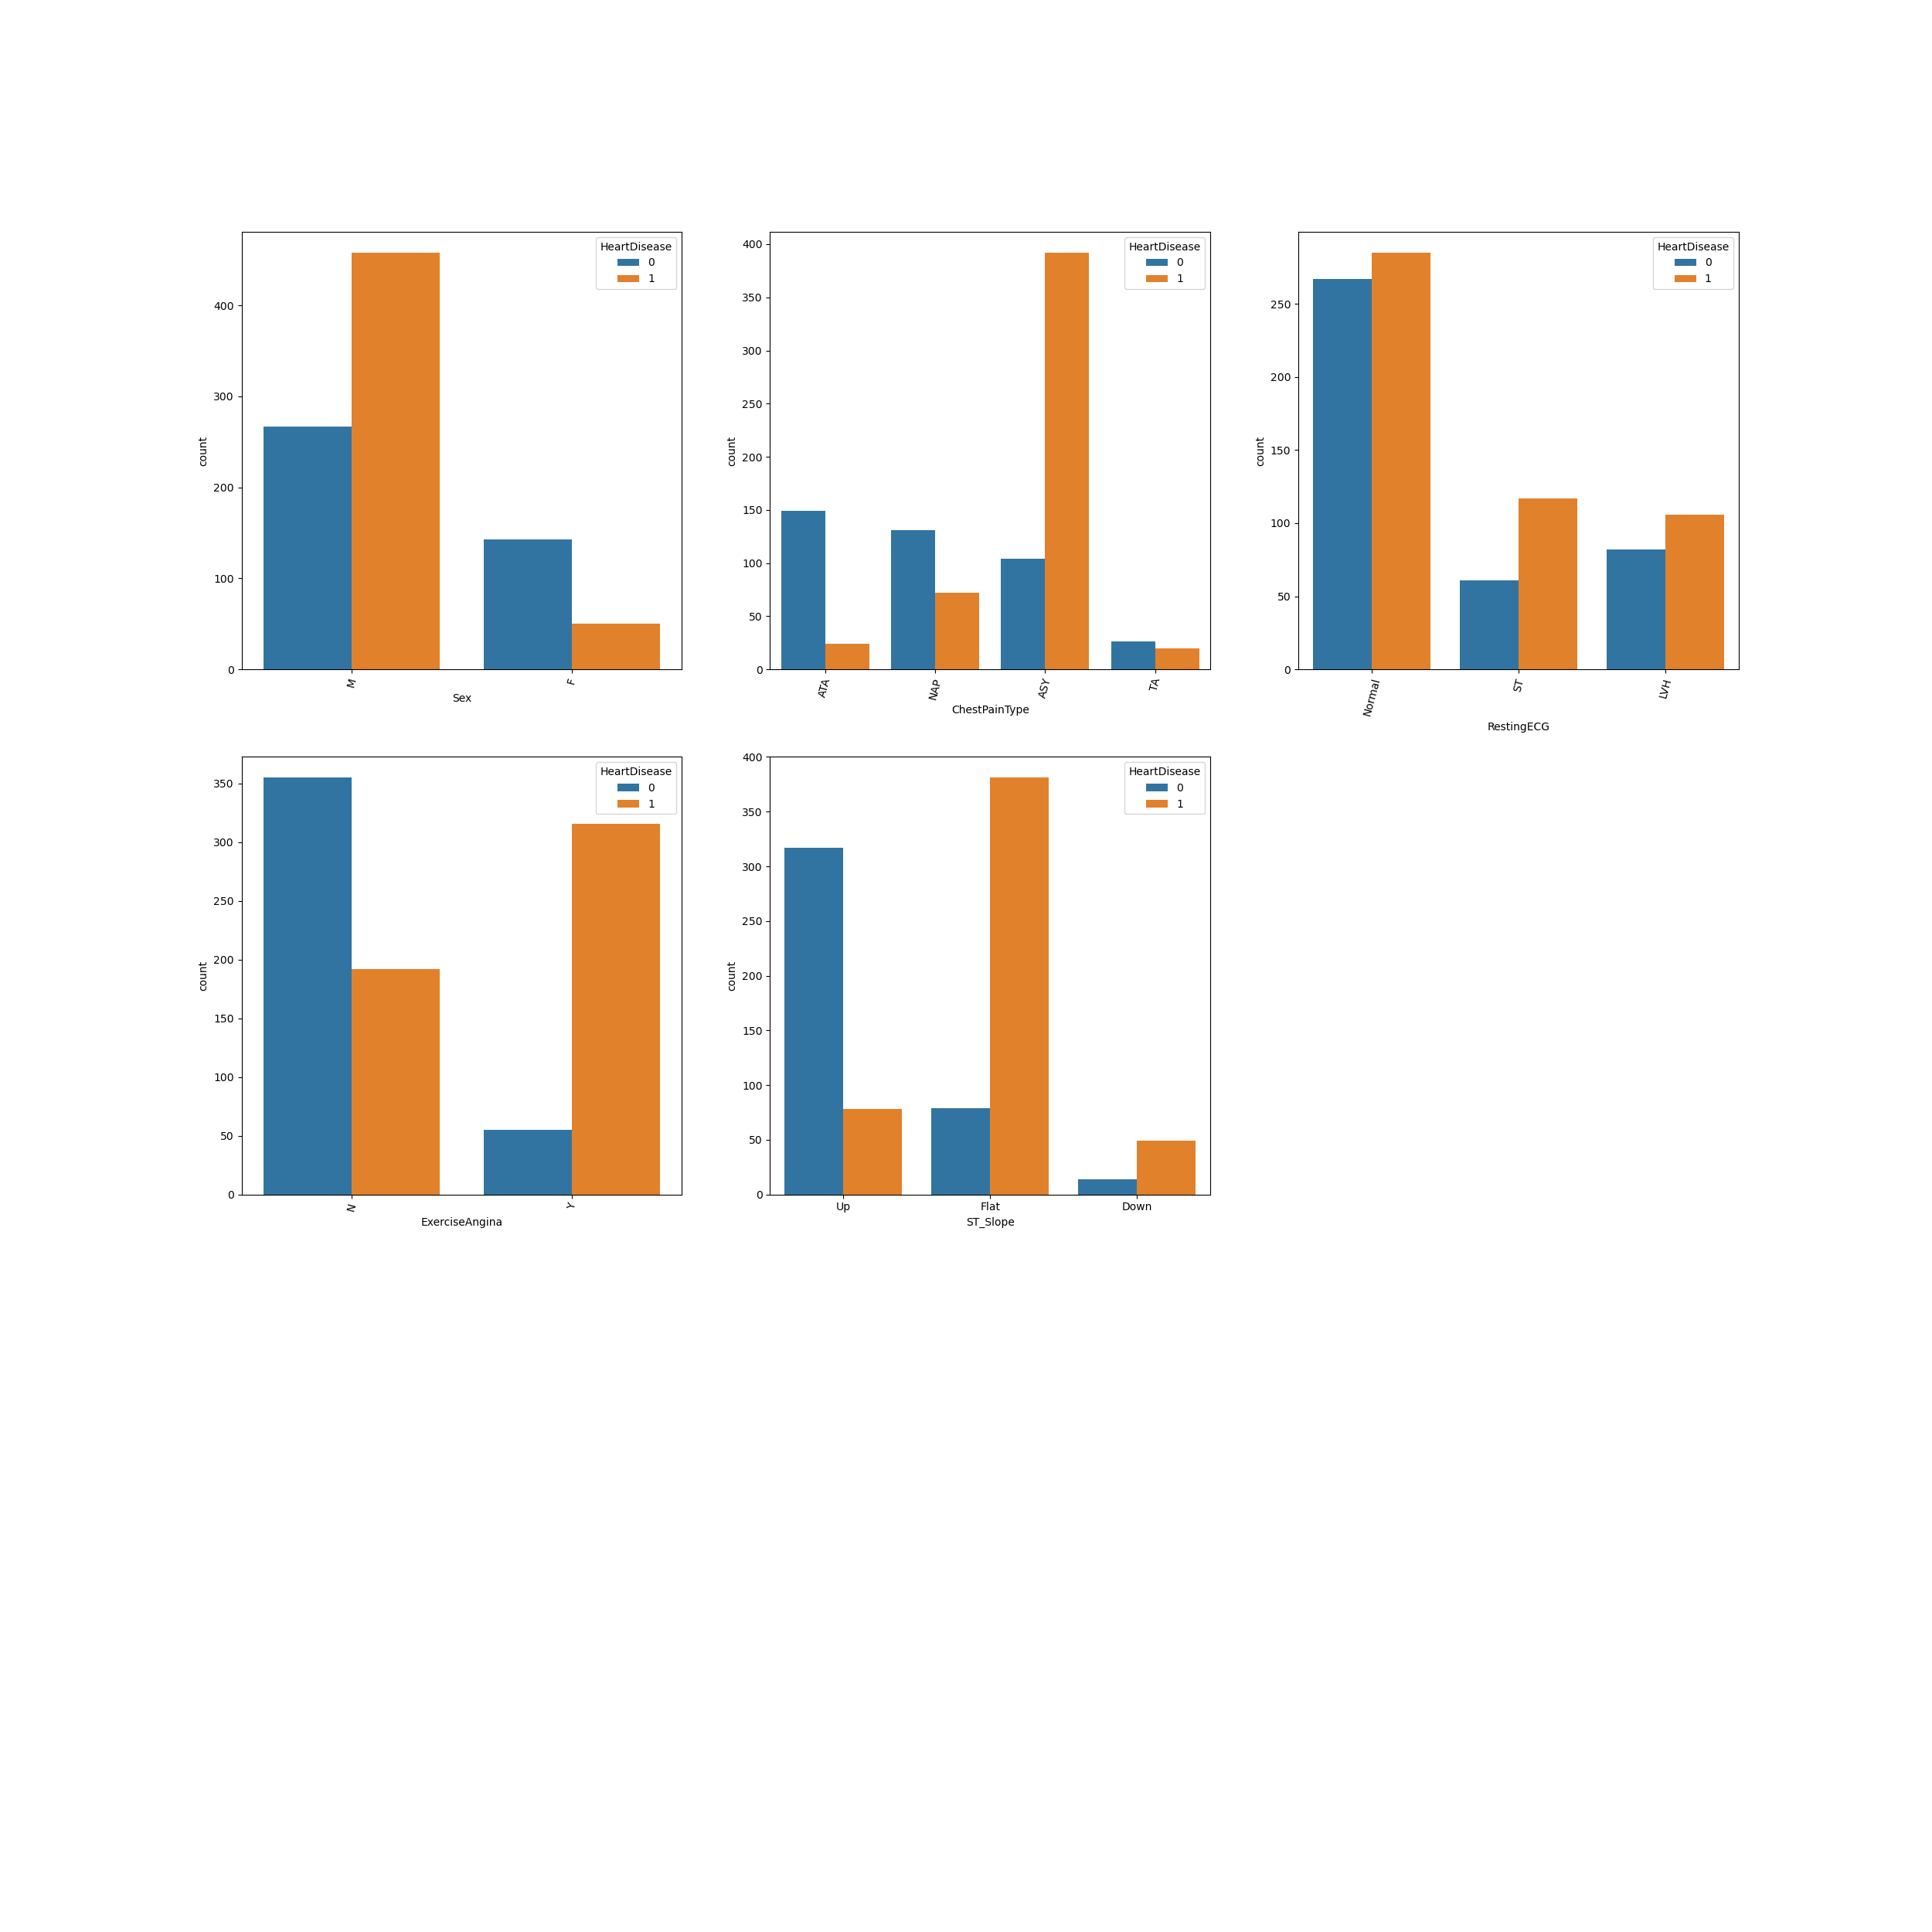
\includegraphics[scale=0.25]{images/heart_cat.png}
\end{figure}


\begin{figure}[H]
     \centering
     \begin{subfigure}[b]{0.3\textwidth}
         \ \caption{Histograma das variáveis numéricas na população total.}
 \label{fig:var:1:card}
 \centering
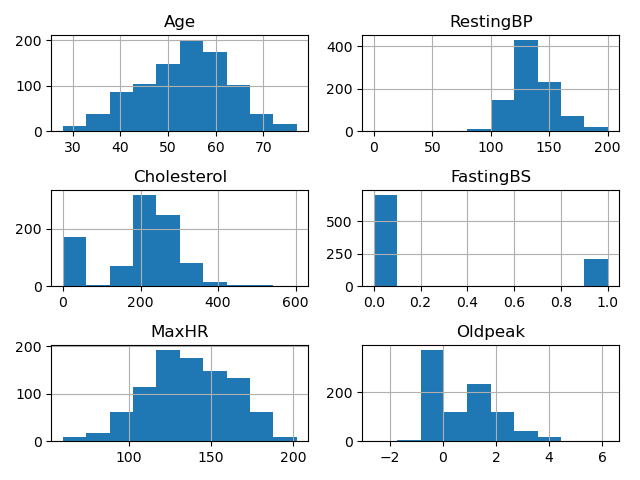
\includegraphics[scale=0.3]{images/hist_heart_t.png}
     \end{subfigure}
     \hfill
     \begin{subfigure}[b]{0.3\textwidth}
         \centering
         \caption{Histograma das variáveis numéricas na população com Insuficiência Cardíaca.}
 \label{fig:var:2:card}
 \centering
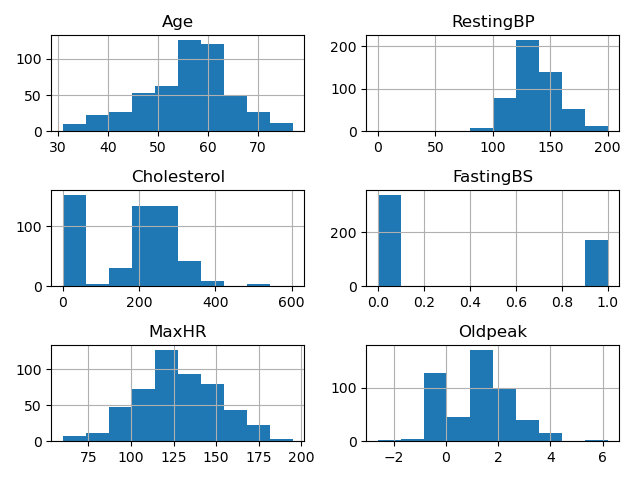
\includegraphics[scale=0.3]{images/hist_heart_yes.png}
     \end{subfigure}
     \hfill
     \begin{subfigure}[b]{0.3\textwidth}
 \caption{Histograma das variáveis numéricas na população sem Insuficiência Cardíaca.}
 \label{fig:var:3:card}
 \centering
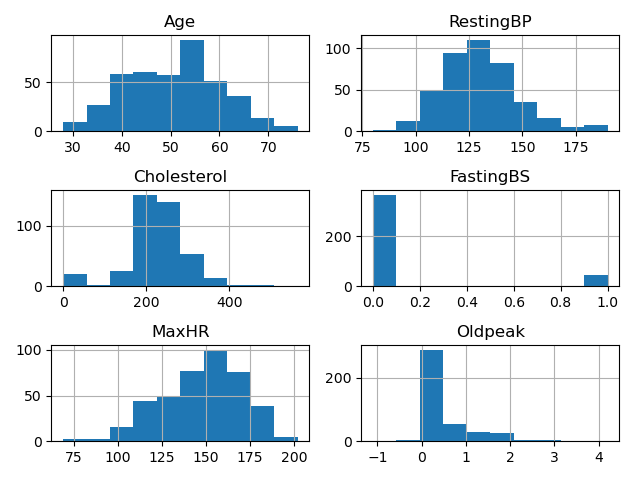
\includegraphics[scale=0.3]{images/hist_heart_no.png}
     \end{subfigure}
        \caption{Distribuição das variáveis numéricas no conjunto de dados de Insuficiência Cardíaca.}
         \label{fig:var:card:t}
\end{figure}

Neste caso iremos transformar as colunas categóricas em ordinais para o conjunto de treinamento nos modelos XGBoost e LightGBM.

\subsection{Cálculo Renal}
O terceiro conjunto de dados é o \href{https://www.kaggle.com/datasets/vuppalaadithyasairam/kidney-stone-prediction-based-on-urine-analysis}{Kidney Stone Prediction based on Urine Analysis}
Este conjunto de dados pode ser usado para prever a presença de cálculos renais com base na análise de urina. As 79 amostras de urina foram analisadas para
determinar se certas características físicas da urina podem estar relacionadas com a
formação de cristais de oxalato de cálcio. Os dados são obtidos de \textit{Physical Characteristics of Urines With and Without Crystals}, Springer Series in Statistics. E as variáveis são:
\begin{itemize}
    \item \textbf{Gravidade Específica:} a densidade da urina em relação à água
    \item \textbf{pH:} pH, o logaritmo negativo do íon hidrogênio.
    \item \textbf{Osmolaridade} uma unidade usada em biologia e medicina, é proporcional à concentração de moléculas em solução.
    \item \textbf{Condutividade:} a condutividade é proporcional à concentração de carga íons em solução.
    \item \textbf{Concentração de Ureia:} concentração de ureia em mm por litro.
    \item \textbf{Concentração de Cálcio} concentração de cálcio.
    \item \textbf{Resultado:} variável alvo (0 ou 1), se possui ou não possui cálculo renal.
\end{itemize}


\begin{table}[H]
\label{descritivo:kindey}
\centering
\begin{tabular}{|c|c|c|}
\hline
\textbf{Coluna} & \textbf{dtypes} & \textbf{\textit{NaN}}\\
\hline
gravity  &  float64 & 0 \\
\hline
ph       &  float64 & 0 \\
\hline
osmo     &    int64 & 0 \\
\hline
cond     &  float64 & 0 \\
\hline
urea     &    int64 & 0 \\
\hline
calc     &  float64 & 0 \\
\hline
target   &    int64 & 0 \\
\hline
\end{tabular}
\caption{Tabela com o tipo de cada variável e quantidade de linhas \textit{NaN} em cada coluna no conjunto de dados de Insuficiência Renal.}
\end{table}
\begin{table}[H]
\label{descritivo:kindey2}
\centering
\begin{tabular}{|c|c|c|c|c|c|c|c|}
\hline
& \textbf{gravity}	& \textbf{ph}	& \textbf{osmo}	& \textbf{cond} & \textbf{urea}	 & \textbf{calc}	 &\textbf{target} \\
\hline
\textbf{count}	& 79.000	& 79.000	& 79.000	& 79.000	& 79.000	& 79.000	& 79.000 \\
\hline
\textbf{mean}	& 1.018	& 6.028	& 612.848	&  20.814	& 266.405	& 4.139	& 0.430\\
\hline
\textbf{std}	    & 0.007	& 0.724	& 237.515	&  7.939	& 131.255	& 3.260	& 0.498\\
\hline
\textbf{min}	    & 1.005	& 4.760	& 187.000	&  5.100	& 10.000	& 0.170	& 0.000\\
\hline
\textbf{25\%}	& 1.012	& 5.530	& 413.000	&  14.150	& 160.000	& 1.460	& 0.000\\
\hline
\textbf{50\%}	& 1.018	& 5.940	& 594.000	&  21.400	& 260.000	& 3.160	& 0.000\\
\hline
\textbf{75\%}	& 1.023	& 6.385	& 792.000	&  26.550	& 372.000	& 5.930	& 1.000\\
\hline
\textbf{max}	    & 1.040	& 7.940	& 1236.000 &  38.000	& 620.000	& 14.340	& 1.000 \\
 \hline
\end{tabular}
\caption{Estatística descritiva das variáveis numéricas no conjunto de dados de Insuficiência Renal.}
\end{table}
\begin{figure}[H]
 \caption{População com Insuficiência Renal e sem Insuficiência Renal.}
 \label{fig:pop:targ:kindney}
 \centering
 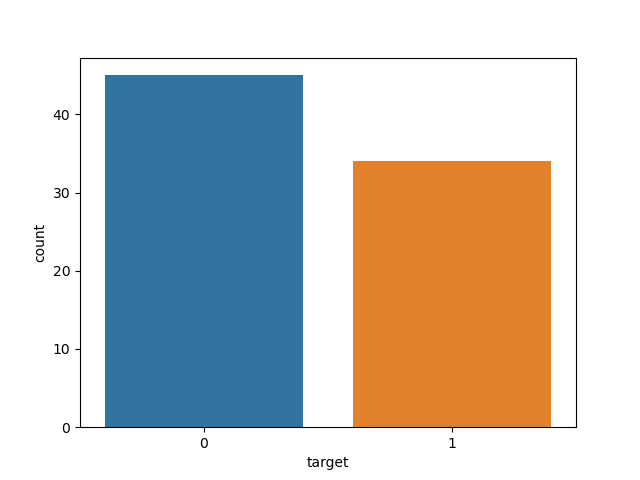
\includegraphics[scale=0.3]{images/kindey_tot.png}
\end{figure}


\begin{figure}[H]
     \centering
     \begin{subfigure}[b]{0.3\textwidth}
         \ \caption{Histograma das variáveis numéricas na população total.}
 \label{fig:var:1:kindney}
 \centering
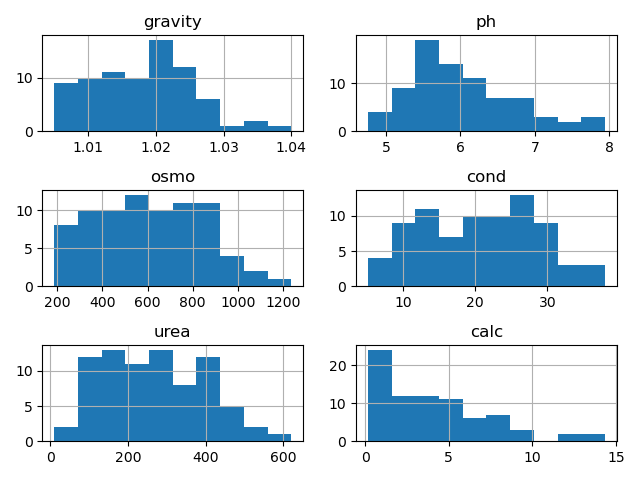
\includegraphics[scale=0.3]{images/hist_kindey_t.png}
     \end{subfigure}
     \hfill
     \begin{subfigure}[b]{0.3\textwidth}
         \centering
         \caption{Histograma das variáveis numéricas na população com Insuficiência Renal.}
 \label{fig:var:2:kindney}
 \centering
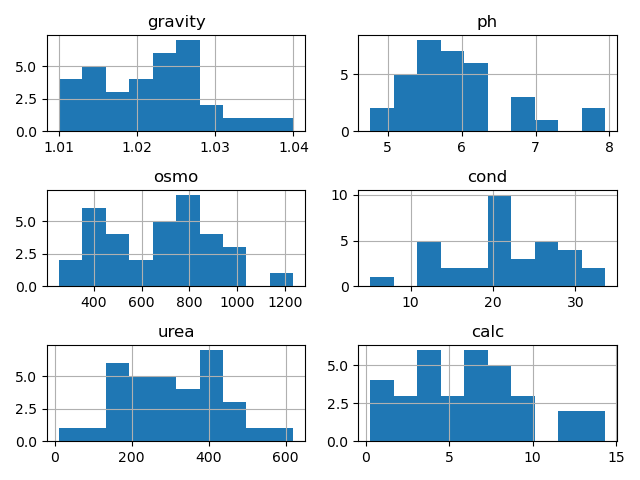
\includegraphics[scale=0.3]{images/hist_kindey_yes.png}
     \end{subfigure}
     \hfill
     \begin{subfigure}[b]{0.3\textwidth}
 \caption{Histograma das variáveis numéricas na população sem Insuficiência Renal.}
 \label{fig:var:3:kindney}
 \centering
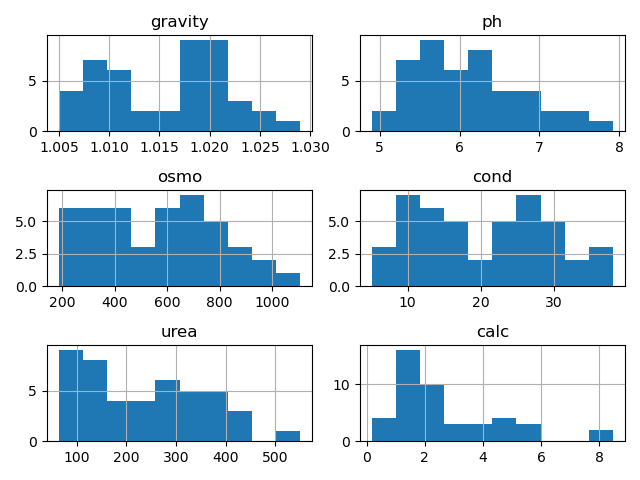
\includegraphics[scale=0.3]{images/hist_kindey_no.png}
     \end{subfigure}
        \caption{Distribuição das variáveis numéricas no conjunto de dados de Insuficiência Renal.}
         \label{fig:var:kindney:t}
\end{figure}

Neste conjunto de dados todos os valores das colunas já são numéricos e não tem \textit{missing}, nenhum tratamento para os dados será necessário. Podendo já utilizar eles na construção dos modelos.
\subsection{Carcinoma da Mama}
O quarto conjunto de dados é o \href{https://www.kaggle.com/datasets/uciml/breast-cancer-wisconsin-data}{Breast Cancer Wisconsin (Diagnostic) Data Set}. Esse conjunto de dados possui características calculadas a partir de uma imagem digitalizada de um aspirado com agulha fina (PAAF) de uma massa mamária. Eles descrevem características dos núcleos celulares presentes na imagem. E o objetivo é diagnosticar o carcinoma da mama como benigno ou maligno.
\begin{itemize}
    \item \textbf{Raio:} média das distâncias do centro aos pontos do perímetro.
    \item \textbf{Textura:} desvio padrão dos valores da escala de cinza.
    \item \textbf{Perímetro:} perímetro calculado para cada núcleo celular
    \item \textbf{Área:} área calculada para cada núcleo celular
    \item \textbf{Suavidade:} variação local nos comprimentos dos raios.
    \item \textbf{Compacidade:} perímetro$^2$ / área - 1,0.
    \item \textbf{Dimensão Fractal:} "aproximação da costa" - 1
    \item \textbf{Simetria:} perímetro$^2$ / área - 1,0.
    \item \textbf{Pontos Côncavos:} número de porções côncavas do contorno.
    \item \textbf{Diagnóstico:} M = maligno, B = benigno.
\end{itemize}

\begin{table}[H]
\label{descritivo:cancer}
\centering
\begin{tabular}{|c|c|c|}
\hline
\textbf{Coluna} & \textbf{dtypes} & \textbf{\textit{NaN}}\\
\hline
id                         &  int64 & 0 \\
\hline
diagnosis                  & object & 0 \\
\hline
radius\_mean               & float64 & 0 \\
\hline
texture\_mean             &  float64 & 0 \\
\hline
perimeter\_mean           &  float64 & 0 \\
\hline
area\_mean               &   float64 & 0 \\
\hline
smoothness\_mean          &  float64 & 0 \\
\hline
compactness\_mean         &  float64 & 0 \\
\hline
concavity\_mean          &   float64 & 0 \\
\hline
concave points\_mean      &  float64 & 0 \\
\hline
symmetry\_mean            &  float64 & 0 \\
\hline
fractal\_dimension\_mean   &  float64 & 0 \\
\hline
radius\_se                &  float64 & 0 \\
\hline
texture\_se              &   float64 & 0 \\
\hline
perimeter\_se            &   float64 & 0 \\
\hline
area\_se                 &   float64 & 0 \\
\hline
smoothness\_se           &   float64 & 0 \\
\hline
compactness\_se          &   float64 & 0 \\
\hline
concavity\_se            &   float64 & 0 \\
\hline
concave points\_se       &   float64 & 0 \\
\hline
symmetry\_se             &   float64 & 0 \\
\hline
fractal\_dimension\_se   &    float64 & 0 \\
\hline
radius\_worst           &    float64 & 0 \\
\hline
texture\_worst         &     float64 & 0 \\
\hline
perimeter\_worst       &     float64 & 0 \\
\hline
area\_worst            &     float64 & 0 \\
\hline
smoothness\_worst      &     float64 & 0 \\
\hline
compactness\_worst     &     float64 & 0 \\
\hline
concavity\_worst       &     float64 & 0 \\
\hline
concave points\_worst  &     float64 & 0 \\
\hline
symmetry\_worst        &     float64 & 0 \\
\hline
fractal\_dimension\_worst   & float64 & 0 \\
\hline
\end{tabular}
\caption{Tabela com o tipo de cada variável e quantidade de linhas \textit{NaN} em cada coluna no conjunto de dados de Carcinoma da Mama.}
\end{table}
\begin{figure}[H]
 \centering
        \caption{Estatística descritiva das variáveis numéricas no conjunto de dados de Carcinoma da Mama.}
         \label{fig:var:cancer:desc}
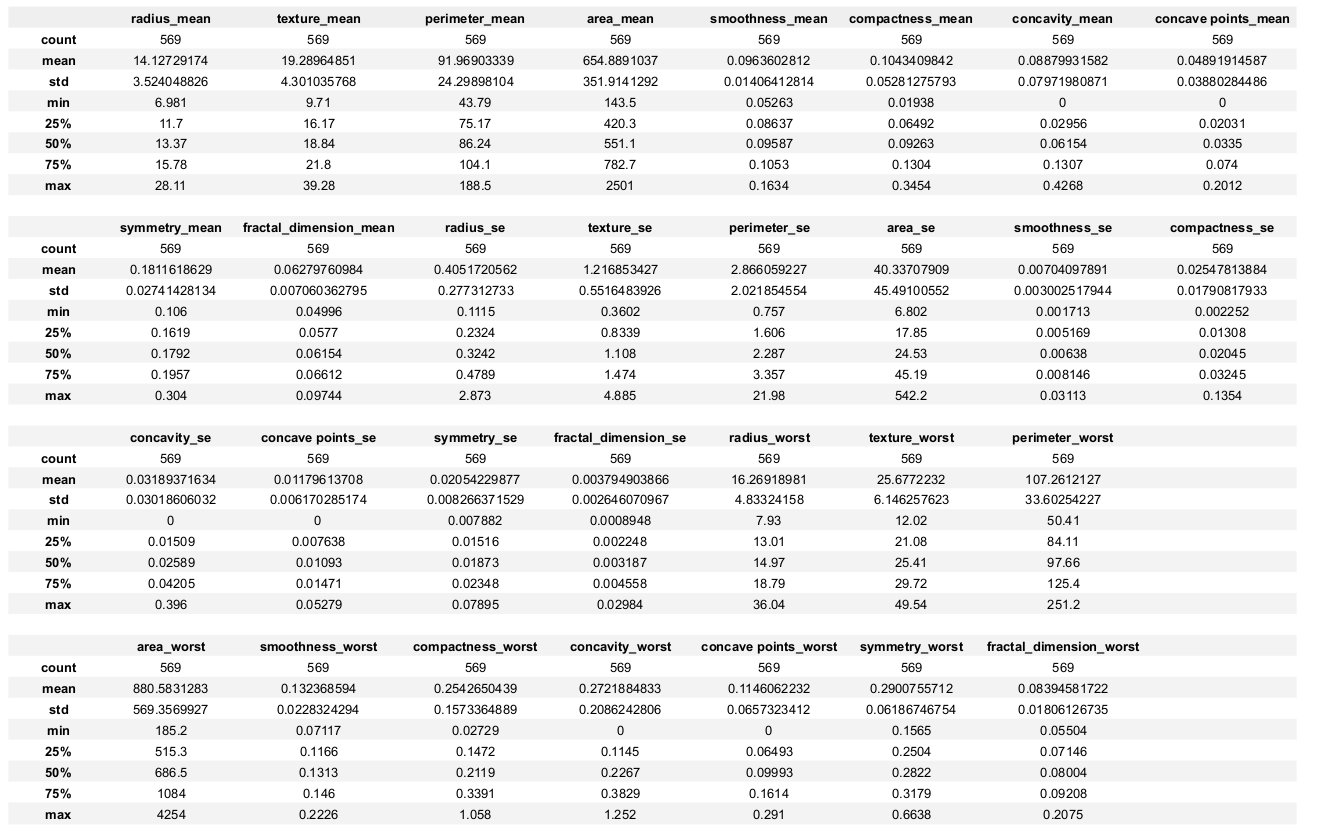
\includegraphics[scale=0.3]{images/descritiva_cancer.png}
\end{figure}
\begin{figure}[H]
 \centering
        \caption{Distribuição de Carcinoma da Mama Maligno e Benigno na população.}
         \label{fig:var:cancer:tot:pop}
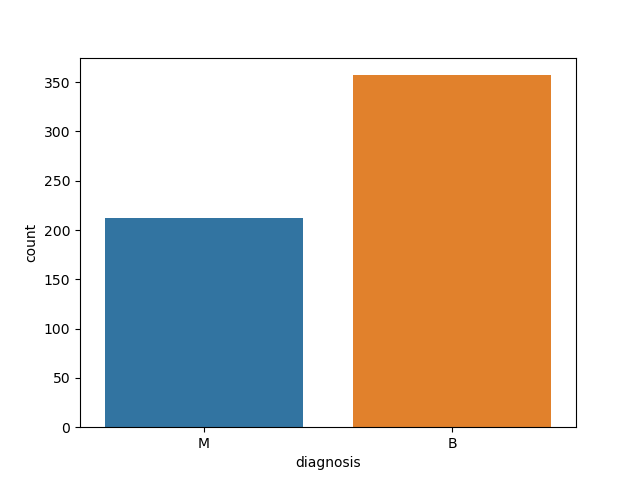
\includegraphics[scale=0.3]{images/cancertot.png}
\end{figure}

\begin{figure}[H]
     \centering
     \begin{subfigure}[b]{0.3\textwidth}
 \centering
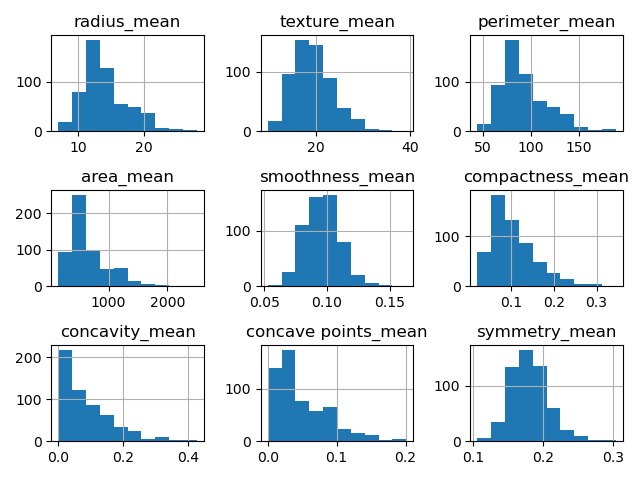
\includegraphics[scale=0.3]{images/hist_cancer_t.png}
     \end{subfigure}
     \hfill
     \begin{subfigure}[b]{0.3\textwidth}
         \centering
 \centering
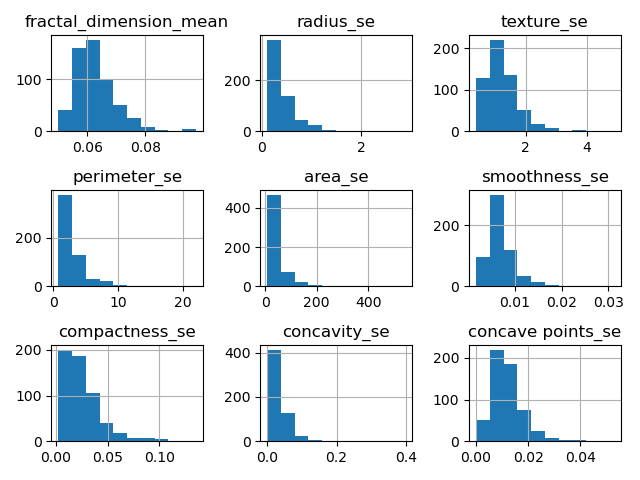
\includegraphics[scale=0.3]{images/hist_cancer_t_2.png}
     \end{subfigure}
     \hfill
     \begin{subfigure}[b]{0.3\textwidth}
 \centering
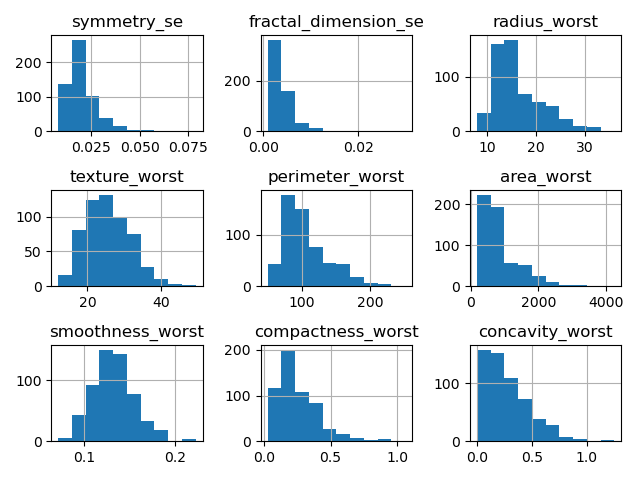
\includegraphics[scale=0.3]{images/hist_cancer_t_3.png}
     \end{subfigure}
          \hfill
     \begin{subfigure}[b]{0.3\textwidth}
 \centering
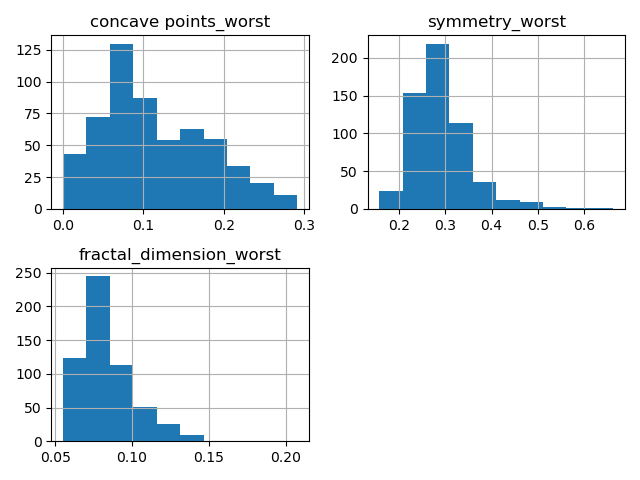
\includegraphics[scale=0.3]{images/hist_cancer_t_4.png}
     \end{subfigure}
        \caption{Distribuição das variáveis numéricas no conjunto de dados de Carcinoma da Mama.}
         \label{fig:var:cancer:t}
\end{figure}

\begin{figure}[H]
     \centering
     \begin{subfigure}[b]{0.3\textwidth}
 \centering
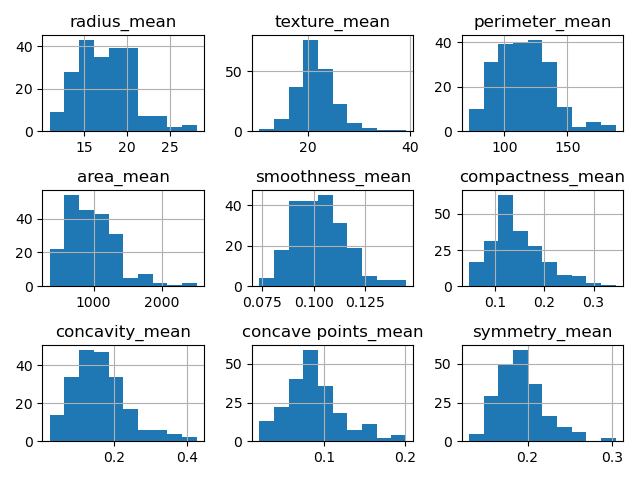
\includegraphics[scale=0.3]{images/hist_cancer_yes_1.png}
     \end{subfigure}
     \hfill
     \begin{subfigure}[b]{0.3\textwidth}
         \centering
 \centering
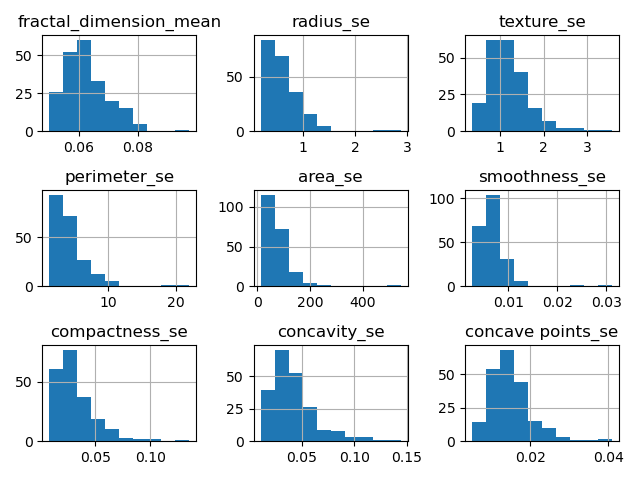
\includegraphics[scale=0.3]{images/hist_cancer_yes_2.png}
     \end{subfigure}
     \hfill
     \begin{subfigure}[b]{0.3\textwidth}
 \centering
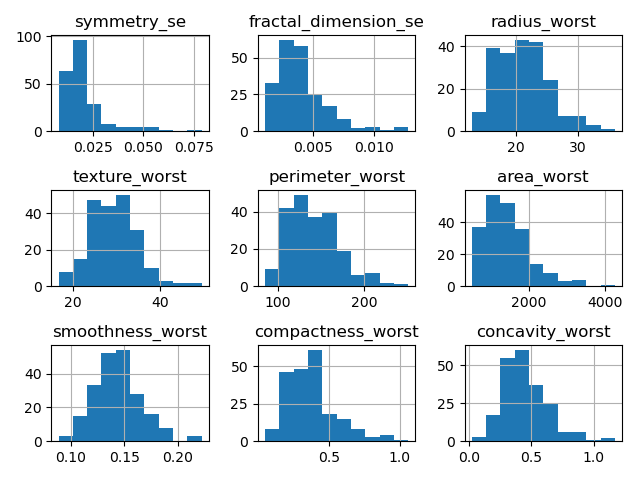
\includegraphics[scale=0.3]{images/hist_cancer_yes_3.png}
     \end{subfigure}
          \hfill
     \begin{subfigure}[b]{0.3\textwidth}
 \centering
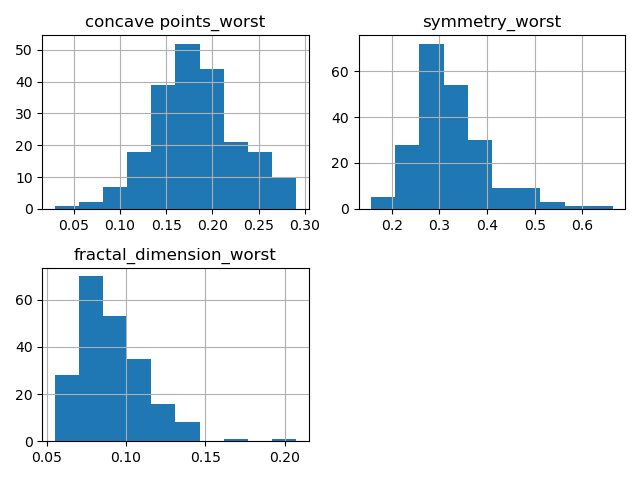
\includegraphics[scale=0.3]{images/hist_cancer_yes_4.png}
     \end{subfigure}
        \caption{Distribuição das variáveis numéricas no conjunto de dados da população com Carcinoma da Mama Maligno.}
         \label{fig:var:cancer:m}
\end{figure}

\begin{figure}[H]
     \centering
     \begin{subfigure}[b]{0.3\textwidth}
 \centering
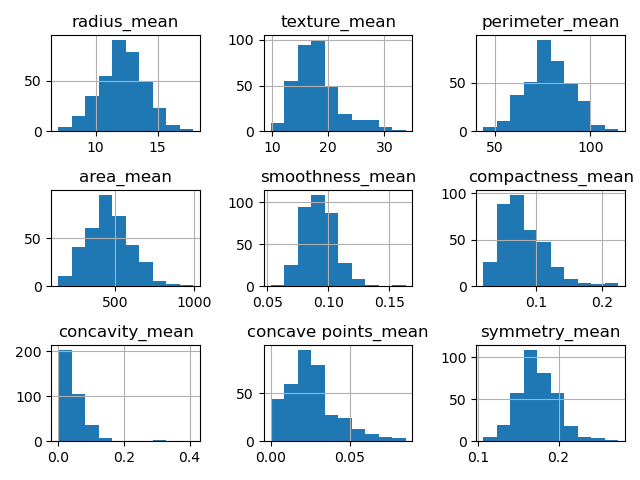
\includegraphics[scale=0.3]{images/hist_cancer_no_1.png}
     \end{subfigure}
     \hfill
     \begin{subfigure}[b]{0.3\textwidth}
         \centering
 \centering
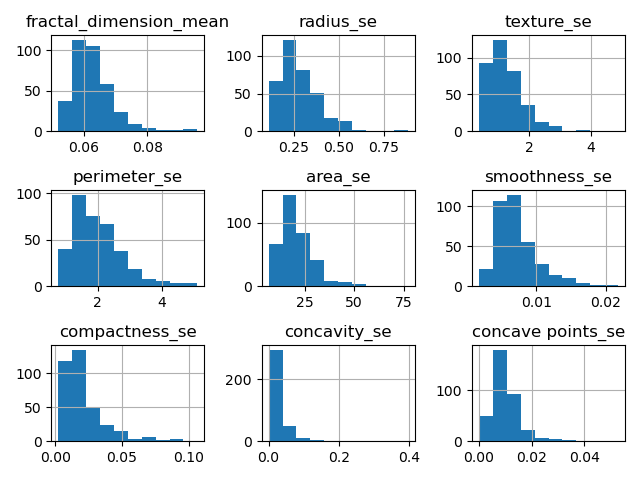
\includegraphics[scale=0.3]{images/hist_cancer_no_2.png}
     \end{subfigure}
     \hfill
     \begin{subfigure}[b]{0.3\textwidth}
 \centering
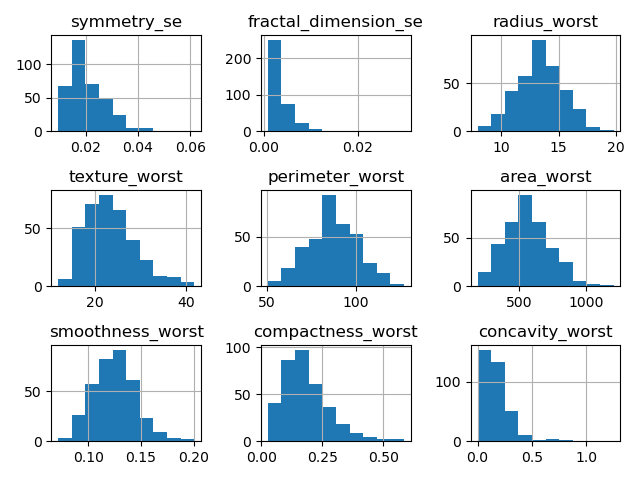
\includegraphics[scale=0.3]{images/hist_cancer_no_3.png}
     \end{subfigure}
          \hfill
     \begin{subfigure}[b]{0.3\textwidth}
 \centering
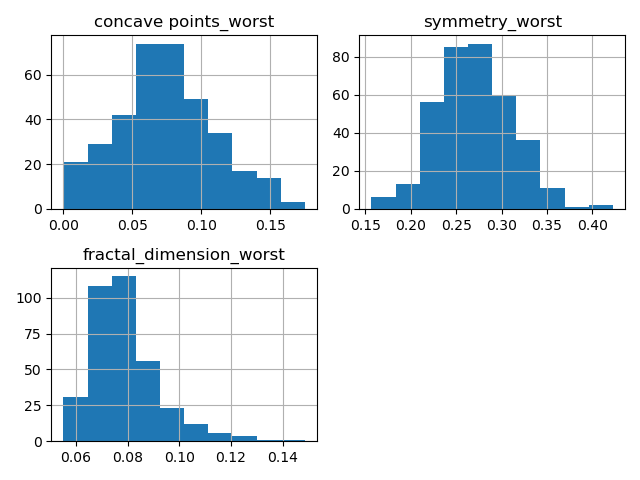
\includegraphics[scale=0.3]{images/hist_cancer_no_4.png}
     \end{subfigure}
        \caption{Distribuição das variáveis numéricas no conjunto de dados da população com Carcinoma da Mama Benigno.}
         \label{fig:var:cancer:b}
\end{figure}


Neste conjunto de dados é necessário criar a variável target 0 ou 1 a partir da coluna
\textbf{diagnosis} e a remoção da coluna \textbf{Unnamed: 32} do conjunto de dados. Após isso os dados já podem ser utilizados para o treino dos modelos preditivos.

\section{Métricas de Validação de Performance e Desempenho}
Para as métricas de performance, utilizamos a AUC, logloss e o KS. O código CITAR mostra a implementação em python dessas métricas.
\begin{codigo}[caption={Código implementado o cálculo da AUC, logloss e o KS.}, label={codigo:im:auc:ks:log}, language=Python, breaklines=true]
def auc_logloss_ks(y_test, y_prob):
    '''
    Input:
        y_prob: model predict prob
        y_test: target
    Output: Metrics of validation
        auc, ks, log_loss
    '''
    fpr, tpr, thresholds = metrics.roc_curve(y_test, y_prob)
    auc = metrics.auc(fpr, tpr)
    log_loss = sklearn.metrics.log_loss(y_test, y_prob)
    ks = max(tpr - fpr)
    return auc, log_loss, ks
\end{codigo}

Para o custo computacional, utilizou-se a biblioteca \textbf{timeit} para o cálculo em nanosegundos. Basta iniciar antes do treino de cada modelo e no final teremos o tempo calculado. O código \ref{codigo:ex:timeit} exemplifica o processo.
\begin{codigo}[caption={Importação da biblioteca timeit e o cálculo em segundos da execução do código.}, label={codigo:ex:timeit}, language=Python, breaklines=true]
import timeit
start = timeit.default_timer()
model_XGB = train(X_train, y_train, X_test, y_test, balanced='balanced', method='XGBoost', number_trials=100)
stop = timeit.default_timer()
stop - start
\end{codigo}

\section{Divisão de Treino e Teste}
Iremos utilizar a função \textit{train\_test\_split} do \textbf{sklearn} para separar o nosso conjunto de treino e teste. $\text{X}$ representa as variáveis explicativas que entraram no treino do modelo e o $y$ representa a variável resposta, target. Não será utilizado o conjunto de validação, pois temos pouco volume de dados em alguns conjunto de dados.

Para os conjunto de dados que possuem apenas dados numéricos será utilizado o mesmo conjunto de treino e teste para todos os modelos, enquanto que os conjunto de dados que possuem variáveis categóricas serão divididos em um conjunto de dados só numéricos para o XGBoost e LightGBM e outro conjunto com variáveis numéricas e categóricas para o CatBoost.
\begin{codigo}[caption={Exemplo da divisão dos conjuntos de treino e teste.}, label={codigo:ex:trainteste_split}, language=Python, breaklines=true]
X_train, X_test, y_train, y_test = train_test_split(X, y, test_size=0.3, random_state=42)
\end{codigo}

\section{Espaço de Hiperparâmetros}
Conforme abordado em \ref{cap3:hiper}, temos alguns parâmetros que são comuns para os três algoritmos, nesta primeira parte do estudo em que vamos alterar os hiperparâmetros manualmente vamos focar neles: \textbf{learning\_rate , max\_depth, n\_estimators, reg\_lambda}. Vamos denotar os hiperparâmetros respectivamente como $LR$, \simbolo{MD}{max\_depth, hiperparâmetro da profundidade máxima}$MD$, \simbolo{RegL}{reg\_lambda, hiperparâmetro da regularização $L_2$}$RegL$. E os valores que vamos testar são:

\begin{gather*}
    LR = \{0.1,0.3\}\\
    MD = \{3,6\}\\
    RegL = \{0.01,0.05\}
\end{gather*}
\section{Tuning do modelo com o Optuna}
Para o tuning com o Optuna foi criada a função objetivo, tuning e o train, de forma que a existência de variáveis categóricas no conjunto de dados já é identificada e, para o caso do \textit{CatBoost}, as separada automaticamente.

O código \ref{codigo:im:tuning} mostra todos os parâmetros das funções e o espaço dos hiperparâmetros que o Optuna irá percorrer para realizar o processo de tuning em cada um dos algoritmos diferentes. Foi utilizado 1 hora como o tempo máximo para o Optuna tunar cada algoritmo, ou seja, cada conjunto de dados demorou cerca de 3 horas para obter os resultados finais.

\begin{codigo}[caption={Código implementado para o Tuning com o Optuna.}, label={codigo:im:tuning}, language=Python, breaklines=true]
import numpy as np
import pandas as pd
import xgboost as xgb
import sys
import timeit
import gc
import sklearn
import seaborn

from sklearn import metrics
from xgboost import XGBClassifier
from catboost import CatBoostClassifier
from sklearn.model_selection import train_test_split
import lightgbm
from lightgbm import LGBMClassifier
from sklearn.metrics import roc_auc_score
from sklearn.metrics import accuracy_score
import optuna
from sklearn.model_selection import GridSearchCV
import matplotlib.pylab as plt
from sklearn.model_selection import cross_val_score
from sklearn.model_selection import StratifiedKFold
from optuna.visualization import plot_optimization_history
from optuna.visualization import plot_param_importances

def auc_logloss_ks(y_test, y_prob):
    '''
    Input:
        y_prob: model predict prob
        y_test: target
    Output: Metrics of validation
        auc, ks, log_loss
    '''
    fpr, tpr, thresholds = metrics.roc_curve(y_test, y_prob)
    auc = metrics.auc(fpr, tpr)
    log_loss = sklearn.metrics.log_loss(y_test, y_prob)
    ks = max(tpr - fpr)
    return auc, log_loss, ks

def objective(trial, X_train, y_train, X_test, y_test, balanced, method):
    '''
    Input:
        trial: trial of the test
        X_train:
        y_train:
        X_test:
        y_test:
        balanced:balanced or None
        method: XGBoost, CatBoost or LGBM
    Output: Metrics of validation
        auc, ks, log_loss
        auc_logloss_ks(y_test, y_pred)[0]
    '''
    gc.collect()
    if method=='LGBM':
        param_grid = {'learning_rate': trial.suggest_float('learning_rate', 0.0001, 0.1, log=True),
                      'num_leaves': trial.suggest_int('num_leaves', 2, 256),
                      'lambda_l1': trial.suggest_float("lambda_l1", 1e-8, 10.0, log=True),
                      'lambda_l2': trial.suggest_float("lambda_l2", 1e-8, 10.0, log=True),
                      'min_data_in_leaf': trial.suggest_int('min_data_in_leaf', 5, 100),
                      'max_depth': trial.suggest_int('max_depth', 5, 64),
                      'feature_fraction': trial.suggest_float("feature_fraction", 0.4, 1.0),
                      'bagging_fraction': trial.suggest_float("bagging_fraction", 0.4, 1.0),
                      'bagging_freq': trial.suggest_int("bagging_freq", 1, 7),
  
                     }
        model = LGBMClassifier(**param_grid)

        print('LGBM - Optimization using optuna')
        model.fit(X_train, y_train)
        
        y_pred = model.predict_proba(X_test)[:,1]

    if method=='CATBoost':
        param_grid = {'learning_rate': trial.suggest_float('learning_rate', 0.0001, 0.1, log=True),
                      'depth': trial.suggest_int("depth", 4, 10),
                      'max_bin': trial.suggest_int('max_bin', 200, 400),
                      'min_data_in_leaf': trial.suggest_int('min_data_in_leaf', 1, 300),
                      'l2_leaf_reg': trial.suggest_float('l2_leaf_reg', 1e-8, 10, log = True),
                      'random_seed': 42,
                      'random_strength': trial.suggest_float("random_strength", 1e-8, 10.0, log=True),
                      'bagging_temperature': trial.suggest_float("bagging_temperature", 0.0, 10.0),
                      'od_type': trial.suggest_categorical("od_type", ["IncToDec", "Iter"]),
                      'od_wait': trial.suggest_int("od_wait", 10, 50),
                     }
        if len(X_train._get_numeric_data().columns) != len(X_train.columns):
            categorical_features_indices = list(X_train.select_dtypes(exclude='number').columns)
            model = CatBoostClassifier(**param_grid)
            print('CATBoost - Optimization using optuna')
            model.fit(X_train, y_train,cat_features=categorical_features_indices,verbose=False)
            y_pred = model.predict_proba(X_test)[:,1]
        else:
            model = CatBoostClassifier(**param_grid)
            print('CATBoost - Optimization using optuna')
            model.fit(X_train, y_train,verbose=False)
            y_pred = model.predict_proba(X_test)[:,1]
        
    if method=='XGBoost':
        param_grid = {'learning_rate': trial.suggest_float('learning_rate', 0.0001, 0.1, log=True),
                      'max_depth': trial.suggest_int('max_depth', 3, 16),
                      'min_child_weight': trial.suggest_int('min_child_weight', 1, 300),
                      'gamma': trial.suggest_float('gamma', 1e-8, 1.0, log = True),
                      'alpha': trial.suggest_float('alpha', 1e-8, 1.0, log = True),
                      'lambda': trial.suggest_float('lambda', 0.0001, 10.0, log = True),
                      'colsample_bytree': trial.suggest_float('colsample_bytree', 0.1, 0.8),
                      'booster': 'gbtree',
                      'random_state': 42,
                     }
        model = XGBClassifier(**param_grid)
        print('XGBoost - Optimization using optuna')
        model.fit(X_train, y_train,verbose=False)
        y_pred = model.predict_proba(X_test)[:,1]
    
    auc_res, log_loss_res, ks_res = auc_logloss_ks(y_test, y_pred)
    print('auc:'+str(auc_res),', log_loss:'+str(log_loss_res),', ks:'+str(ks_res))
    return auc_logloss_ks(y_test, y_pred)[0]

def tuning(X_train, y_train, X_test, y_test, balanced, method):
    '''
    Input:
        trial: 
        x_train:
        y_train:
        X_test:
        y_test:
        balanced:balanced or not balanced
        method: XGBoost, CatBoost or LGBM
    Output: Metrics of validation
        auc, ks, log_loss
        auc_logloss_ks(y_test, y_pred)[0]
    '''
    study = optuna.create_study(direction='maximize', study_name=method+' Classifier')
    func = lambda trial: objective(trial, X_train, y_train, X_test, y_test, balanced, method)
    print('Starting the optimization')
    time_max_tuning = 60*30 # max time in seconds to stop
    study.optimize(func, timeout=time_max_tuning)
    return study

def train(X_train, y_train, X_test, y_test, balanced, method):
    '''
    Input:
        X_train:
        y_train:
        X_test:
        y_test:
        balanced:balanced or None
        method: XGBoost, CatBoost or LGBM
    Output: predict model
    '''
    print('Tuning')
    study = tuning(X_train, y_train, X_test, y_test, balanced, method)
    if method=='LGBM':
        model = LGBMClassifier(**study.best_params)
        print('Last Fit')
        model.fit(X_train, y_train, eval_set=[(X_test,y_test)],
                 callbacks = [lightgbm.early_stopping(stopping_rounds=100), lightgbm.log_evaluation(period=5000)])
    if method=='CATBoost':
        model = CatBoostClassifier(**study.best_params)
        if len(X_train._get_numeric_data().columns) != len(X_train.columns):
            categorical_features_indices = list(X_train.select_dtypes(exclude='number').columns)
            print('Last Fit')
            model.fit(X_train, y_train,cat_features=categorical_features_indices, eval_set=[(X_test,y_test)],
                 early_stopping_rounds=100,verbose = False)
        else:
            print('Last Fit')
            model.fit(X_train, y_train, eval_set=[(X_test,y_test)],
                 early_stopping_rounds=100,verbose = False)
    if method=='XGBoost':
        model = XGBClassifier(**study.best_params)
        print('Last Fit')
        model.fit(X_train, y_train, eval_set=[(X_test,y_test)],
                 early_stopping_rounds=100,verbose = False)
    return model, study
\end{codigo}

\section{Explicabilidade dos Modelos}
Para as versões finais de cada modelo, que são aquelas que obtiveram as melhores métricas de performance, iremos aplicar os Valores de SHAP para realizar a explicabilidade de cada variável e seu impacto no modelo final.

O código \ref{codigo:ex:shap} demonstra como é a execução do SHAP.
\begin{codigo}[caption={Importação da biblioteca shap e o cálculo dos shap values.}, label={codigo:ex:shap}, language=Python, breaklines=true]
import shap
explainer = shap.TreeExplainer(model_XGB)
shap_values = explainer.shap_values(X_train)
shap.summary_plot(shap_values, X_train,plot_size=.7)
\end{codigo}




